\documentclass[a4paper,10pt,titlepage]{report}

\usepackage[utf8]{inputenc}
\usepackage[T1]{fontenc}
\usepackage[english]{babel}
\usepackage{amssymb}
\usepackage{amsmath}
\usepackage{amsthm}
\usepackage{graphicx}
\usepackage{fancyhdr}
\usepackage{lastpage}
\usepackage{listings}
\usepackage{algorithm}
\usepackage{algpseudocode}
\usepackage[document]{ragged2e}
\usepackage[margin=1in]{geometry}
\usepackage{enumitem}
\usepackage{color}
\usepackage{datenumber}
\usepackage{venndiagram}
\usepackage{chngcntr}
\usepackage{mathtools}
\usepackage{booktabs}
\setcounter{tocdepth}{4}
\DeclarePairedDelimiter{\ceil}{\lceil}{\rceil}

%lstlisting ting:
\definecolor{dkgreen}{rgb}{0,0.45,0}
\definecolor{gray}{rgb}{0.5,0.5,0.5}
\definecolor{mauve}{rgb}{0.30,0,0.30}
\lstset{frame=tb,
  language=C,
  aboveskip=3mm,
  belowskip=3mm,
  showstringspaces=false,
  columns=flexible,
  basicstyle={\small\ttfamily},
  numbers=left,
  numberstyle=\footnotesize,
  keywordstyle=\color{dkgreen}\bfseries,
  commentstyle=\color{dkgreen},
  stringstyle=\color{mauve},
  frame=single,
  breaklines=true,
  breakatwhitespace=false
  tabsize=1
}
\lstset{literate=%
{æ}{{\ae}}1
{å}{{\aa}}1
{ø}{{\o}}1
{Æ}{{\AE}}1
{Å}{{\AA}}1
{Ø}{{\O}}1
}
\lstset{extendedchars=\true}
\lstset{inputencoding=ansinew}
\renewcommand{\lstlistingname}{Code}

\setdatetoday
\addtocounter{datenumber}{0} %date for dilierry standard is today
\setdatebynumber{\thedatenumber}
\date{}


\setcounter{section}{-1}
\setcounter{tocdepth}{3}
\setcounter{secnumdepth}{2}


\pagestyle{fancy}
\fancyhf{}
\title{CC - Assignment 3}

\newcommand{\Z}{\mathbb{Z}}
\lhead{Compiler (DM546)}
\rhead{Mjerv15, Trpet15  \& Mojae15}
\rfoot{Page  \thepage \, of \pageref{LastPage}}
\counterwithin*{equation}{section}

\begin{document}
\newpage
{%
\centering
    \huge
    \bfseries
    \vspace{5mm}
CC, Spring 2018\\
Exam project, part 3\\
\vspace{5mm}
\begin{tabular}{|l|l|}
\hline
Group & 1 \\ \hline
\end{tabular}
\\
\vspace{10mm}
\begin{tabular}{@{}ll@{}}
\toprule
\multicolumn{1}{|l|}{Name}      & \multicolumn{1}{l|}{Mark Wolff Jervelund } \\ \midrule
\multicolumn{1}{|l|}{Birthday}  & \multicolumn{1}{l|}{280795} \\ \midrule
\multicolumn{1}{|l|}{Login}     & \multicolumn{1}{l|}{mjerv15@student.sdu.dk} \\ \midrule
\multicolumn{1}{|l|}{Signature} & \multicolumn{1}{l|}{\includegraphics[scale=0.3]{img/mark_sign}} \\ \midrule
                                &                       \\ \midrule
\multicolumn{1}{|l|}{Name}      &  \multicolumn{1}{l|}{Troels Blicher Petersen} \\ \midrule
\multicolumn{1}{|l|}{Birthday}      &   \multicolumn{1}{l|}{230896} \\ \midrule
\multicolumn{1}{|l|}{Login}      &  \multicolumn{1}{l|}{trpet15@student.sdu.dk} \\ \midrule
\multicolumn{1}{|l|}{Signature}      & \multicolumn{1}{l|}{\includegraphics[scale=0.08]{img/troels_sign} } \\ \midrule
                                &                       \\ \midrule
\multicolumn{1}{|l|}{Name}     &  \multicolumn{1}{l|}{Morten Kristian Jæger} \\ \midrule
\multicolumn{1}{|l|}{Birthday}      &  \multicolumn{1}{l|}{030895} \\ \midrule
\multicolumn{1}{|l|}{Login}     &   \multicolumn{1}{l|}{mojae15@student.sdu.dk} \\ \midrule
\multicolumn{1}{|l|}{Signature}    &  \multicolumn{1}{l|}{\includegraphics[scale=0.3]{img/morten_sign}} \\ \midrule
\end{tabular}
\\
\vspace{10mm}
This report contains a total of \underline{ \pageref{LastPage} } pages.
}

\begin{titlepage}
\centering
    \vspace*{9\baselineskip}
    \huge
    \bfseries
    3. Assignment \\
    \normalfont
    Mark Jervelund, Troels Blicher Petersen \& Morten Jæger  \\
    (Mjerv15, Trpet15, Mojae15) \\
	\huge
    Compiler (DM546)  \\[4\baselineskip]
    \normalfont
	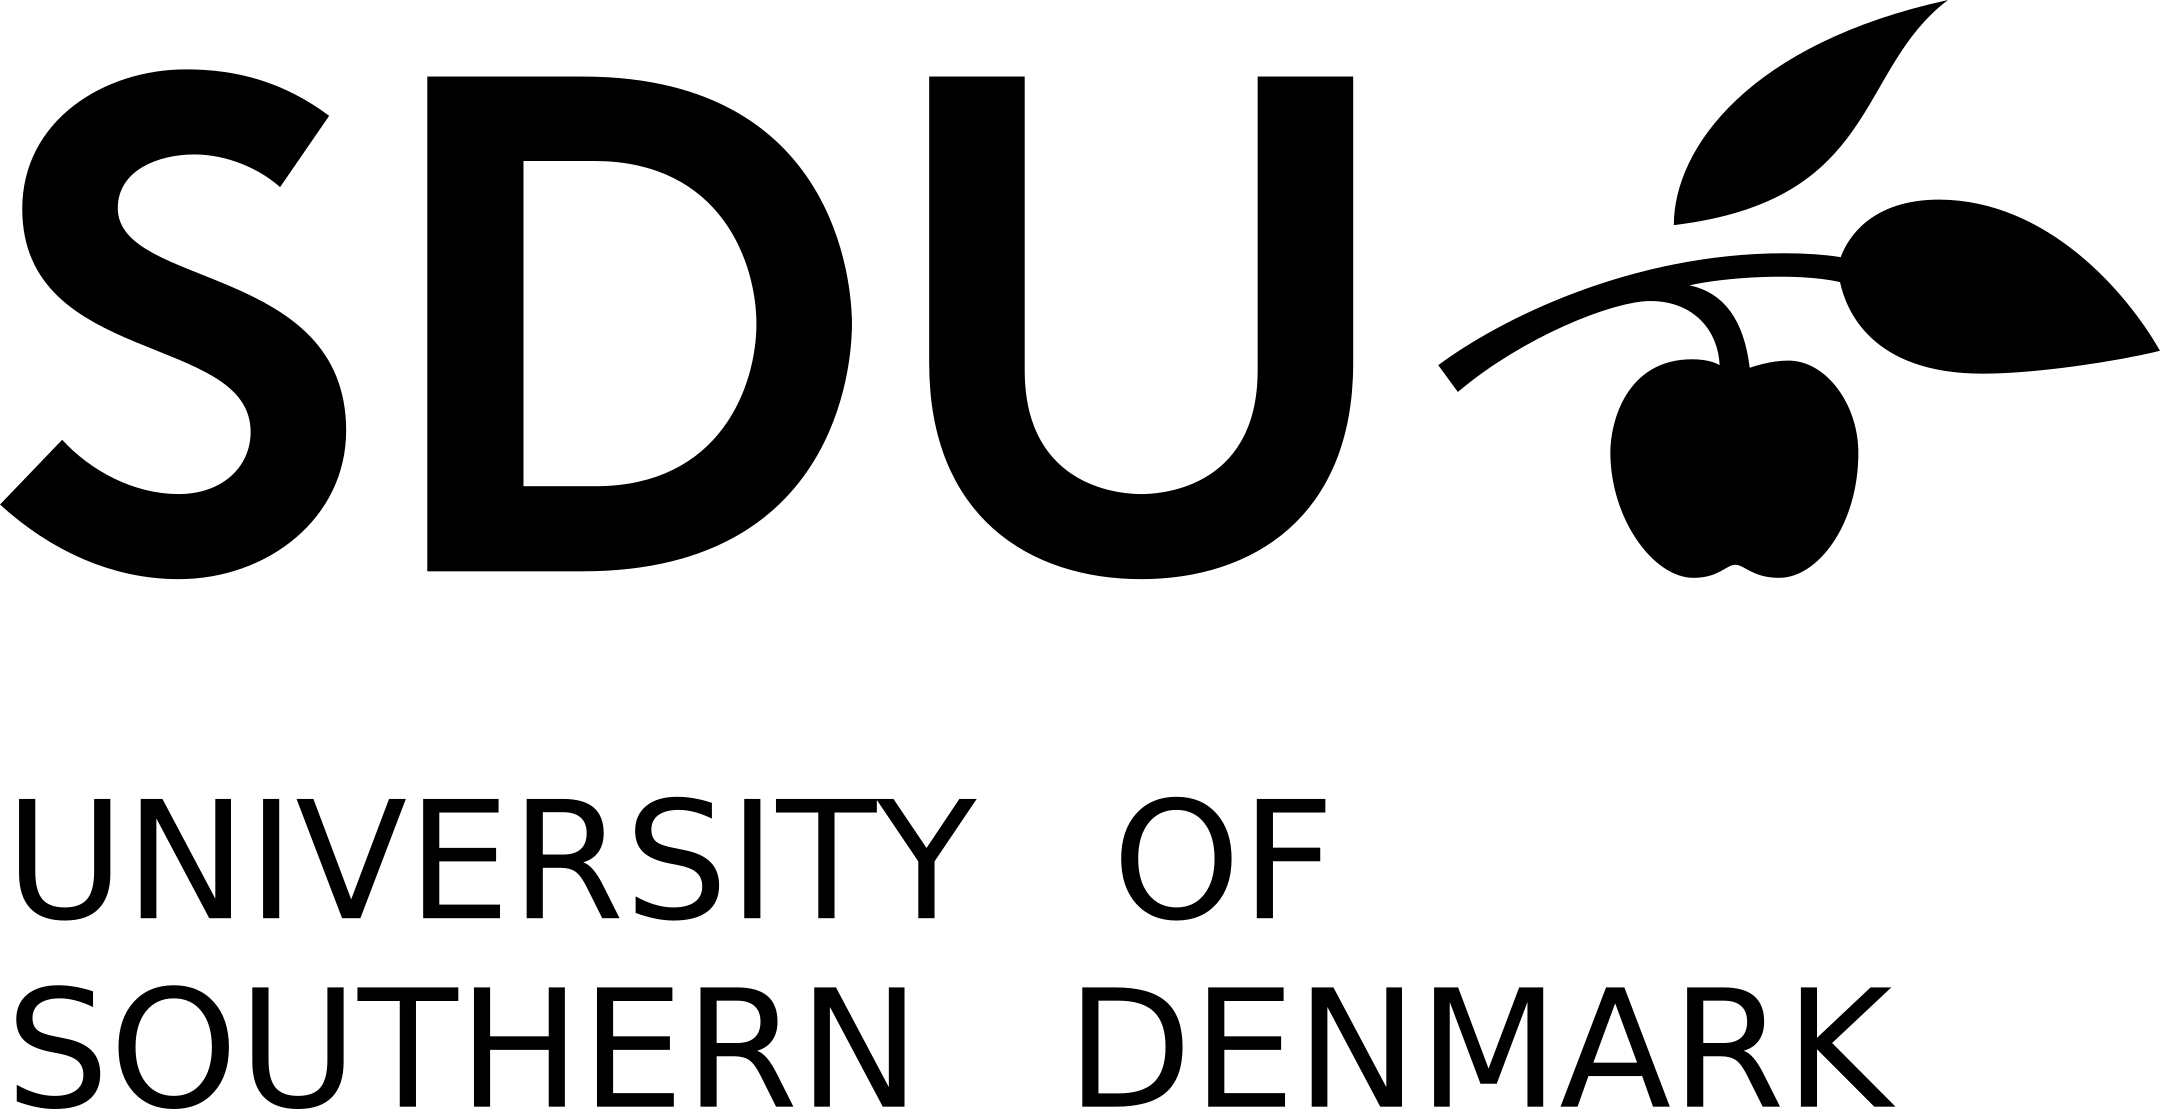
\includegraphics[scale=1]{img/SDU_logo}
    \vfill\
    \vspace{5mm}
    IMADA \\

    \textbf{\datedate} \\[2\baselineskip]
\end{titlepage}

\renewcommand{\thepage}{\roman{page}}%
\tableofcontents
\newpage
\setcounter{page}{1}
\renewcommand{\thepage}{\arabic{page}}


\newpage

\section{Introduction}

\subsection{Clarifications}

\subsection{Limitations}

\subsection{Extensions}

\subsection{Implementation Status}

\section{Parsing and Abstract Syntax Trees}
\section{Begin old}
\section{Introduction}
In the second task of the Compiler project, we are tasked with implementing a Scanner and a Parser, using Flex and Bison, and a Pretty printer. This is all to be done in C. As part of the project, all the files needed to complete the project were given beforehand, and only needed to be edited. An essential part of this project, is to implement an Abstract Syntax Tree, to give the compiler a way of understanding the code.

\subsection{How to compile and run}
Besides the main objective of this assignment, the group has also started implementing a more modular project structure, which will be explained in the design section. However, a brief introduction on how to build and run the program will be given here.\\
\vspace{6px}
Since the program is already starting to take modular shape, there are several ways to compile it. The easiest way is to simply run in the directory of the \textsf{Makefile}
\begin{lstlisting}
make all
\end{lstlisting}
\textsf{make all} will, however, build all binaries. Including the ones from Assignment 1. Therefore, for this project it is also possible to simply run
\begin{lstlisting}
make exp
\end{lstlisting}
This will only compile and output the program \textsf{exp} for this assignment. Before running the program \textsf{exp}, it is important to have the input file in the same directory.\\
\vspace{6px}
There are two ways to run the program \textsf{exp}. The first is to simply run
\begin{lstlisting}
./exp
\end{lstlisting}
This will run the program and read an input file \textsf{input.txt}. The other way to run the program is by passing the file to test on the command line, as an argument.
\begin{lstlisting}
./exp <inputfile>
\end{lstlisting}
This makes it a little easier to test several different testcases, without having to change the same file all the time.\\
\vspace{6px}
To remove all object files, run
\begin{lstlisting}
make clean
\end{lstlisting}
To remove all object files and executable binaries, run
\begin{lstlisting}
make clean-all
\end{lstlisting}

\section{Design} %%TODO SKAL NOK OGSÅ VÆRE NOGET OM ABSTRACT SYNTAX TREE
\subsection{Scanner and Parser}
The scanning and parsing is the main subject in this report. It is here the written program (to be compiled) is pulled apart to understand its structure and meaning.
\subsubsection{Scanner}
The scanner needs to be able to recognize the different symbols that are specified in the assignment. This means that it needs to be able to spot and return the different operators we are working with (+, -, /, *, etc.), and the specific words as specified in the syntax. These are words like, "while", "if", "array of", and such. After spotting these symbols, the scanner needs to pass them on to the parser, which will parse the input, and start creating our Abstract Syntax Tree. \\
\vspace{6px}
Another feature of the scanner, is the possibility to be able to weed out some "bad" programs already at this point. To do this, the scanner checks for input not defined in the language, which means that neither the scanner, nor the parser can do anything with it. If this happens, we want to be able to tell the user, that the program is not valid. The scanner should also check whether multi-line comments have been closed by the end on the program, as this is also not legal, according to the grammar of the language.

\subsubsection{Parser}
The parser needs to be a able to recognize the input it gets from the scanner, and match that up with the grammar of the language. This means that it needs to be able to match the input from the scanner, with the rules in the grammar. When the parser matches some input with one of the rules, it should create a node in our Abstract Syntax Tree, which we can use later on, f.x. for printing the AST.\\
\vspace{6px}
Another feature of the parser, it the possibility to weed out some "bad" programs, like we also did in the scanner phase. To do this, the parser checks if a function has the same name in both the name and the tail. If this is not the case, the user should be notified of the error, just like we did in the scanner phase.

\subsection{Abstract Syntax Tree (AST)}
The abstract syntax tree is a datastructure used to keep track of the way, the program we read, is built. The AST is built from the parser, which, given some input from the scanner, matches the input with the rules of the language, and creates nodes in the AST. An example of how a node could be created, is when the parser reads some input with a "+" between two expressions. The parser would then create a node in the AST, which would be a "+"-node. This node would then have two child nodes, which would the the expressions on each side of the "+" symbol. This is the way we build up our AST when we parse the input.

\subsection{Pretty Printer}
The pretty printer needs to be able to print the Abstract Syntax Tree we get from parsing the input program. This must be done in such a way, that the corresponding output from the pretty printer looks like the original program as much as possible, assuming that the original program is not weeded out at this point. Small changes to the output does happen however, such as indentation, and parentheses.

\subsection{New Project Structure}
As mentioned in the introduction, the group has implemented a new project structure to accommodate for a more modular design. The main goal is to have all modules separate, so that removing one module in theory would not break the rest. It was also found that the makefile should be easy to use, so that adding new files to a module in most cases would not require any changes to this file. To some degree this might not seem important, but as the project grows larger it might turn out to be a very convenient choice.\\
\vspace{6px}
It has been chosen, that each module will have its own include directory instead of one big shared include directory. This makes it easier to separate the modules, and removing a module is as simple as removing its directory.\\
\vspace{6px}
The project will be built in the build folder, and all module objects will reside in their respective folder, to prevent possible collisions of filenames.


\newpage

\section{Implementation}
\subsection{Scanner and Parser}
\subsubsection{Scanner}

\begin{lstlisting}
/* abbreviation of symbols we match on, TO BE EXPANDED */
SYMBOLS [+\-*\/\(\)\[\]{}!\|,\.=;:]

%%
[ \t]+        /* ignore */;
\n              lineno++;

{SYMBOLS}       return yytext[0];
\end{lstlisting}
Above is a small part of the "exp.l" file, which is the file Flex uses to scan the given program. This code handles the different symbols that we want to match on, when scanning the file. We use an list of all the symbols we can match on, as this was easier than writing each and every symbol out individually.

\begin{lstlisting}
"<="            return LEQ;
">"             return GT;
">="            return GEQ;
"if"            return IF;
"else"          return ELSE;
\end{lstlisting}
Above is another small part, that shows how we return tokens when reading certain words, or symbols.

\begin{lstlisting}
<COMMENT_MULTI>{

\n              lineno++;
"(*"            nested_comment++;
"*)"            {   nested_comment--;
                    if (nested_comment == 0){
                        BEGIN(0);
                    }
                }
.               /* ignore */
<<EOF>>         fprintf(stderr, "Comment not closed at the end of the file. Found at line: %i\n", lineno); exit(1);
}
\end{lstlisting}
Above is the part of the scanner that takes care of multi-line comments. The state for multi-line comments check for nested comments, and, as described in the design section, returns an error if the comment is not closed by the end of the file.

\subsubsection{Parser}
\begin{lstlisting}
expression  :   expression '+' expression
        {$$ = make_EXP(exp_PLUS, $1, $3);}
            | expression '-' expression
        {$$ = make_EXP(exp_MIN, $1, $3);}
            | expression '*' expression
        {$$ = make_EXP(exp_MULT, $1, $3);}
            | expression '/' expression
        {$$ = make_EXP(exp_DIV, $1, $3);}
            | '(' expression ')'
        {$$ = $2;}
\end{lstlisting}
Above is a small part of the "exp.y" file, which is the file Bison uses for parsing the input from the scanner. This part of the code is a part of the code that handles expressions, by making nodes in the AST.
\begin{lstlisting}
function    :   head body tail
        {$$ = make_Func($1, $2, $3);
        if (check_Func($1, $3) != 0){
            fprintf(stderr, "Function name: %s, at line %i, does not match function name: %s, at line %i\n", $1->id, $1->lineno, $3->id, $3->lineno);
            YYABORT;
            }}
;
\end{lstlisting}
As described in the design section, we want to check if a function has the same name in the head and the tail. This part of the code checks this, by calling the function "check\_func()". This function checks the "id" of the given head and tail. If they are not equal, we give the user an error message, stop the parsing, since the input program is not valid.
\subsection{Abstract Syntax Tree}
\begin{lstlisting}
expression *make_EXP(EXP_kind kind, expression *left, expression *right){
    expression *e;
    e = NEW(expression);
    e->lineno = lineno;
    e->kind = kind;
    e->val.ops.left = left;
    e->val.ops.right = right;
    return e;
}
\end{lstlisting}
Above is a small part of the functions used to create the AST. This particular function is used to create expressions, with an expression on each side of an operator. This operator could be "+", "-", "*", and so on. As described in the design section, when we create this node, we set the left and right side of the operator as the children of the node.

\subsection{Pretty Printer}
\begin{lstlisting}
void prettyEXP(expression *e) {
    switch (e->kind) {

        case exp_MULT:
            prettyEXP(e->val.ops.left);
            printf("*");
            prettyEXP(e->val.ops.right);
            break;

        case exp_DIV:
            prettyEXP(e->val.ops.left);
            printf("/");
            prettyEXP(e->val.ops.right);
            break;
\end{lstlisting}
The code above is a part of the function used to print expressions. The way this is done, is by checking the expressions "kind", which describes what kind of expression we are working with. When we know what kind of expression we have, we can print the expression with the correct operators

\subsection{New Project Structure}
Implementation of this new structure is fairly simple. However, it was chosen to divide the scanner, parser and pretty printer into separate modules. This approach is a little backwards in terms of the new modular design, since they appear to heavily depend on each other. But, it also means that it is possible to remove one module and replace it with another if need be.

\section{Testing}
The programs used to test the scanner, parser, and pretty printer can be found in the appendix. Some are simple, to just test the basics of the program, and some are more complicated (contain unary minus, expressions with absolute values which looks like "||"). The programs are not meant to be run as actual programs, so they may not make sense.
\section{Results}
\subsection{Test1}
This is just a basic test, to make sure indentation works and such.
\begin{lstlisting}
func test(n : int) : int
    return 2;
end test
write test();
\end{lstlisting}

\subsection{Test2}
We now test if we can handle unary minuses.
\begin{lstlisting}
func test(n : int) : int
    if (n == 0 || n == 1) then
        return -1;
 else
        return n*factorial(n-1);
end test
write test();
\end{lstlisting}

\subsection{Test3}
We now test if we can handle an absolute value expression that looks like an "or" 
\begin{lstlisting}
func test(n : int) : int
    if (n == 0 || n == 1 || ||a+b|+c|) then
        return -1;
 else
        return n*factorial(n-1);
end test
write test();
\end{lstlisting}

\subsection{Test4}
We now test if we get an error if the function name is not the same in the head and the tail of the function.
\begin{lstlisting}
Function name: test, at line 2, does not match function name: nottest, at line 4
Segmentation fault (core dumped)
\end{lstlisting}

\subsection{Test5}
We now test if we get an error if we do not close a multi-line comment.
\begin{lstlisting}
Comment not closed at the end of the file. Found at line: 9
\end{lstlisting}

\subsection{Test6}
We now test if we get an error if we read a symbol that is not in our grammar.
\begin{lstlisting}
Unrecognized symbol. Found at line: 7
\end{lstlisting}
\section{Conclusion}
From the tests we have run, we can conclude that our scanner, parser, AST, and pretty printer works as intended on a given program. 



\section{End old}
\subsection{The Grammar}

\subsection{Use of the {\tt flex} Tool}

\subsection{Use of the {\tt bison} Tool}

\subsection{Abstract Syntax Trees}

\subsection{Syntactic Sugar}

\subsection{Weeding}

\subsection{Test}

%%We should write some shit here.
\section{The Symbol Table}
\section{Begin old}
\section{Introduction}
In the first task of the Compiler project we are tasked with implementing a Symbol Table in C. For this we are given skeleton code for the Symbol data structure and the header files for the functions we need to implement.

\section{Design}
The symbol table works like a normal extendible hashing. This is accomplished, by hashing the name of the symbol that has to be inserted, as described in the first part of the project, and putting the symbol into that place in the hash table.\\
The different functions that has been implemented for the symbol table is the following:
\subsubsection{Hash()}
The Hash function hashes a given name for a symbol. This is done according to the project description, where the binary value of the letters are added together, while shifting the bits to the left

\subsubsection{initSymbolTable()}
This function initializes a symbol table, meaning that it allocates the memory needed for the symbol table. Is also "initializes" the list of symbol the table has, by setting these to be "NULL". This is done, to make it easier, to check if there already is a symbol at this place in the list.

\subsubsection{scopeSymbolTable()}
As described in the project description, this function creates a new symbol table. It then points it to the given table, as its "\verb!next!"

\subsubsection{putSymbol()}
The putSymbol function takes a symbol and a table, and tries to insert that symbol into the given table. If the symbol is already in the given table, nothing should be done, as the symbol is already in the table. However, if the symbol is not in the table, it is inserted as the first element in the chaining list for its hash value.

\subsubsection{getSymbol()}
The getSymbol function checks the given table for some given symbol. If the symbol is found, we just return the symbol. If the symbol is not found in the given table, the next table is checked, and so on. This keeps going on either until the symbol is found, or run out of tables.

\subsubsection{dumpSymbolTable()}
The dumpSymbolTable recursively prints the symbols of a given table, and the tables "\verb!next!"




\newpage
\section{Implementation}
\subsection{Hash} 
\begin{lstlisting}
int Hash(char *str) {
    unsigned int length;
    length = (unsigned) strlen(str);
    int k = (int) str[0];
    int i;
    int pointer = 1;
    while (pointer < length) {
        k = k << 1;
        i = (int) str[pointer];
        k = i + k;
        pointer++;
    }
    return (k % HashSize);
}
\end{lstlisting}
The hash function is implemented as listed in the project description. It simply shifts and adds the integer representation of the characters in the input string and adds them. When this is done, the modulo of the result is found, to get an index for the hash table.

\subsection{initSymbolTable}
\begin{lstlisting}
SymbolTable *initSymbolTable() {

    int i = 0;
    SymbolTable *table = Malloc(sizeof(SYMBOL) * HashSize);
    table->next = NULL;
    while (i < HashSize) {
        table->table[i] = NULL;
        i++;
    }
    return table;
}
\end{lstlisting}
As described in the design section, memory is allocated for the symbol table. Then all the elements of the list are set to "NULL", to make is easy to check if there is something at that place in the list. 

\subsection{scopeSymbolTable}
\begin{lstlisting}
SymbolTable *scopeSymbolTable(SymbolTable *t) {
    SymbolTable *newTable = initSymbolTable();
    newTable->next = t;
    return newTable;
}
\end{lstlisting}
As described in the design section, a new table is initialized in the beginning. Afterwards, the table is pointed to the table-argument.

\subsection{putSymbol}
\begin{lstlisting}
SYMBOL *putSymbol(SymbolTable *t, char *name, int value) {
    if( t == NULL ) {
        return NULL;
    }
    SYMBOL *localCheck = checkLocal(t, name);
    //Symbol already exists
    if (localCheck != NULL){
        return localCheck;
    }
    else {

        SYMBOL *symbol = Malloc(sizeof(SYMBOL));
        symbol->name = name;
        symbol->value = value;
        symbol->next = Malloc(sizeof(SYMBOL));

        //Placed in front of the list
        symbol->next = t->table[value];
        t->table[value] = symbol;
        return symbol;

    }
}
\end{lstlisting}
As described in the design section, the current table is checked, using the "\verb!localCheck!" function. If the symbol is not found, it is inserted into the current table. This is done by first making the symbol point to what is currently the first element of the chaining list, and afterwards making the first element in the chaining list point to the symbol, that has to be inserted. This ensures that the symbol, that has to be inserted, is the first in the chaining list, and that it points to the next element in the list.

\subsubsection{checkLocal}
\begin{lstlisting}
SYMBOL *checkLocal(SymbolTable *t, char *name){
    int hashValue = Hash(name);
    
    SYMBOL *symbol = t->table[hashValue];
    if (symbol == NULL){
        return NULL;
    }

    else {
        while (symbol != NULL){
            if (strcmp(name, symbol->name) == 0){
                return symbol;
            }
            symbol = symbol->next;
        }
    }

    //Hash value for the symbol exists, but the symbol is not in the table
    return NULL;
}
\end{lstlisting}
The checkLocal function checks if the given symbol is in the given symbol table. This is done by checking the names of the the symbols in the chaining list, at the place of the proper hash value.

\subsection{getSymbol}
\begin{lstlisting}
SYMBOL *getSymbol(SymbolTable *t, char *name) {
//    First check if t is null
    if (t == NULL) {
        return NULL;
    }

    SYMBOL *localCheck = checkLocal(t, name);

    //Symbol in local table?
    if (localCheck != NULL){
        return localCheck;
    }

    if (t->next != NULL){
        getSymbol(t->next, name);
    }

    //Symbol does not exists
    return NULL;
}
\end{lstlisting}
The getSymbol function checks the current table for a given symbol, by using the checkLocal function. If the symbol is not found in the given table, the table's "\verb!next!" is checked for the symbol.

\subsection{dumpSymboltable}
\begin{lstlisting}
void dumpSymbolTable(SymbolTable *t) {
    if (t == NULL){
        return;
    }

    printf("\t\tPrinting symbol table:\n\n");

    for (int i = 0; i < HashSize; i++) {
        SYMBOL *symbol = t->table[i];
        if (symbol != NULL){
            printf("Hash: \t%i ", i);
            while (symbol != NULL){
                printSymbol(symbol);
                printf(" ");
                symbol = symbol->next;
            }
            printf("\n");
        }
    }
    printf("\n");

    dumpSymbolTable(t->next);
}
\end{lstlisting}
The dumpSymbolTable function prints out the symbols of the table, and what hash value they correspond to. The printout of the symbols is left to the printSymbol function.

\subsubsection{printSymbol}
\begin{lstlisting}
void printSymbol(SYMBOL *symbol){
    printf("(%s, %i)", symbol->name, symbol->value);
}
\end{lstlisting}
The printSymbol function prints out the name and value of a symbol. This is a separate function, to make it easier to add more printouts in the future, while keeping dumpSymbolTable the same.
\newpage
\section{Testing}
To test the implemented functions, a program to run all the tests, was made. In the testing program, the "\verb!value!" of the symbols was the hash value of the name:
\subsection{Test 1 - Testing the Hash function}
The first test is to check the value of the hashing function. This was done using the string "kitty" (in the program refered to as "testString"), which we already know the expected value of.

\subsection{Test 2 - Testing the initSymbolTable}
The second test is to check if we are able to initialize a symbol table for further use. This is done by checking if the returned symbol table is "NULL" or not.

\subsection{Test 3 - Testing the putSymbol function}
The third test is to check if we can put a symbol into our table, and to check if the returned symbol is the one we expected, by comparing it to the "\verb!name!" and "\verb!value!" we put in the putSymbol function

\subsection{Test 4 - Testing the getSymbol function}
The fourth test is to check if we can get a symbol out from the symbol table. This is done by checking if the "\verb!name!" and "\verb!value!" of the symbol we get from the getSymbol function, are the same as the one we used in the putSymbol function.

\subsection{Test 5 - Testing the putSymbolfunction again}
The fifth test is to check if we can put a symbol into the table, which already exists. This is done by using the putSymbol function to insert a symbol which already exists in the table, and check if the returned symbol is correct.

\subsection{Test 6 - Testing the getSymbol function for a symbol which is not in the table, but a symbols with its hash value is}
The sixth test is to check if we get a "NULL" when trying to call getSymbol with a symbol that does not exists in the table, but a symbol with the same value as it, is in the table. This is done by first inserting a symbol that has a certain hash value, and then calling getSymbol of a symbol that has the same hash value, but a different name. If "NULL" is returned, we know that the symbol does not exist in the table.

\subsection{Test 7 - Testing the putSymbolfunction for a symbol which hash is already in the table}
The seventh test is to check if we can insert a symbol in the table, where there already is a symbol at its hash value. This is done by using the symbol we used in test 6, but this time we insert it into the table.

\subsection{Test 8 - Testing the scopeSymbolTable function}
The eighth test is to check if we are able to scope a symbol table. This is done by checking if the returned symbol table is "NULL" or not.

\subsection{Test 9 - Testing the putSymbol function for the new table}
The ninth test is to check if we are able to insert a symbol into the new table we got from test 8. This is done by checking if the symbol we get has the same "\verb!name!" and "\verb!value!" as we put in the putSymbol arguments.
\\~\\
Last we call the dumpSymbolTable function, to see if the symbol table we see here, is what we expected.

\section{Results}
The output of the testing program is as follows:
\begin{lstlisting}
Testing hash function
Test 1 - Hash function test PASSED


Testing init table function
Test 2 - Table constructed PASSED


Testing putsymbol function
Test 3 - Symbol correctly made.


Testing getSymbol function
Test 4 - Symbol correctly returned.


Testing putsymbol function again
Test 5 - Symbol correctly made.


Testing searching for a symbol, that is not in the table, but the hash for the symbol exists.
Test 6 - NULL successfully received.

Testing putSymbol function with a symbol which hash already is in the table
Test 7 - Symbol correctly made.

Testing scopeSymbolTable function
Test 8 - Table constructed PASSED


Testing putsymbol function in new table
Test 9 - Symbol correctly made.


 
Tests PASSED 9

 
		Printing symbol table:

Hash: 	199 (kitty, 199) 

		Printing symbol table:

Hash: 	94 (tets, 94) (tesu, 94) 
Hash: 	199 (kitty, 199) 


\end{lstlisting}

\section{Conclusion}
From our tests we can conclude that the code performs as expected with the expected output.


\section{End Old}

The symbol table works like a standard extendible hash table, It's function is to store our symbols in
\subsection{Scope Rules}

\subsection{Symbol Data}

\subsection{The Algorithm}
\textcolor{red}{Hashing Algorithm ?}

\subsection{Test}
Write test from the other reports. give a example but keep it mainly text based.

\section{Type Checking}
\section{Begin old}

\section{Introduction}
In the third assignment of the Compiler project, we are tasked with implementing a weeder phase and a typechecking phase, with primary focus on the typechecking phase. This entire third assignment in made only in C.

\subsection{Build and execute}
To build and execute first run either \textsf{make}, \textsf{make all} or \textsf{make compiler}.
\begin{lstlisting}
make
\end{lstlisting}
All ways will build the binary called \textsf{compiler}. \\
\vspace{6px}
If one wants debug info from the compiler, this can be added, by uncommenting the \textsf{\#define debugflag} in \textsf{debug.h}.
\begin{lstlisting}
#ifndef COMPILER_DEBUG_H

#define debugflag

#define COMPILER_DEBUG_H
\end{lstlisting}
By having it as a definition in the header file, it ensures that all debug related prints wont get compiled, when building the compiler for production use. However, it comes with the caveat, that the entire project has to be cleaned \textsf{make clean} if this is changed.\\
\vspace{6px}
There are several ways to run the program, all of which can be found by executing the program \textsf{compiler} with the option "\textsf{-h}"
\begin{lstlisting}
./compiler -h
\end{lstlisting}
The program accepts raw text input, in form of a program, as an argument. It also accepts files with the Shere Khan extension \textsf{.src} as an argument. Both ways will in the current state of the compiler return imformation that the compiler has gathered about the program to be compiled.\\
\vspace{6px}
To remove all object files, run
\begin{lstlisting}
make clean
\end{lstlisting}
To remove all object files and executable binaries, run
\begin{lstlisting}
make clean-all
\end{lstlisting}


\section{Design}
The design involves the weeder and the typechecker. The weeder is run before the typechecker, to weed out any errors and potentially find any expressions that can already be 

\subsection{Weeder}
Design of the weeder is similar to that of the parser. However, it differs in that it looks for expressions that can already be evaluated at compile time. This will slow down compilation time, however, it will also allows for some optimizations in the compiled program. \\
At this point our weeder is primarily focused on logical expressions. These are fairly straightforward to evaluate at compile time and also provide increases in performance, since comparing values is usually a "slow" process in processors due the operations itself and branch prediction.\\
\vspace{6px}
Therefore, looking for expressions that evaluate true means, that there is no reason to do that comparison. This not only allows us to remove that if-statement, but it also allows us to remove other parts of the program that cannot be run as a result of this. This could be an if-else-statement, because this code would never be able to run anyways. \\
Same can be said with if-statements that evaluates to false everytime. However, in that case, only the part that evaluates to false can be removed, as other parts of an if-else-statement might still be able to evaluate true.\\
\vspace{6px}
The weeder can also look for virtual constants, that is, variables and expressions which are calculated in some way, but can be calculated already at compile time. This reduces the number of calculations to perform during execution of the program.\\
\vspace{6px}
Lastly, but still very important, is the ability to check whether a function has any return calls. If not, the compiler should hault compiling and report an error, that a return is missing. This will be done using a stack, that keeps track of all returns inside and outside a function. A stack is smart, because it can be used in a way to describe all the contents of a function and scoping.\\
\vspace{6px}
Adding a weeder will increase compile time, since it has to check for all of these things. However, there are many potential performance gains in the compiled program, which makes it a worthwile thing to do. One way to increase the speed of the weeder is to reuse the same tree as the one made by the parser. This way the entire program wont have to be read again and instead the datastructure describing the program can be used.

\subsection{Typechecker}
The thought behind designing the typechecker, was to do this in three parts or phases. These three phases are the \textit{"setup"}, \textit{"pickup"} and "\textit{"check"} phases.

\subsubsection{Setup Phase}
In the setup phase, we go through the AST we have from parsing the program, and setup symbols and symbol tables for the different nodes in the AST.\\
The symbols we insert into our symboltables are f.x. the id of a function, the name of a variable.\\
To help with identifying what a symbols type is when we want to check it later, we have a structure called \textit{"symbol\_type"}, which contains information about the symbol it is in. If the symbol we insert is from a f.x. from a function, this \textit{"symbol\_type"} will also contain information about the functions, like its return type and such.\\
Since this phase is mostly just setting up symboltables and preparing for the "pickup" and "check" phases, this could possibly be used when we create the nodes themselves, and thus save a pass-through of the AST.

\subsubsection{Pickup Phase}
In the pickup phase, we go through the AST again, but this time we try to resolve symbol that doesn't have a specific type yet. An example of this could be the following:
\begin{lstlisting}
type t1 = t2;
type t2 = int;
\end{lstlisting}
When we first go through the AST in the setup phase, we do not know what type \textit{t1} has yet, but when we go through the pickup phase, we resolve these problems. This phase is also used to resolve deeper recursively defined types, and resolve conflicts with these.

\subsubsection{Check Phase}
In the check phase, we go through the AST and, since we should now know the type of everything in the given program, we can do the actual typechecking. The typechecking is done by checking the type we get from the \textit{"symbol\_type"} structure, with what we expect to actually occur. An example of this could be a comparison of two variables:
\begin{lstlisting}
var a : int;
var b : int;
a = 5;
b = 4;
if (a > b) then
write 1;
\end{lstlisting}
In this case, there would be no problems with the typechecking, since we know that to say that a variable is larger than another variable, both of these variable must be integers in this language.\\
However if the program was as follows:
\begin{lstlisting}
var a : int;
var b : bool;
a = 5;
b = true;
if (a > b) then
write 1;
\end{lstlisting}
We would get an error, since the two types are incompatible, according to our language.

\section{Implementation}

\subsection{Weeder}
\begin{lstlisting}
 if ((left_term->kind == term_NUM) && (right_term->kind == term_NUM)){
            //We have an expression with two constants
            switch(expression->kind){

                case (exp_MULT):
                    temp = make_Term_num(left_term->val.num * right_term->val.num);
                    break;
\end{lstlisting}
Above is a small part of the weeding program, where we decide what to do if an expression consists of two numbers. In this case, we have a multiplication, which we can then resolve in compile time, instead of having to generate code for this calculation later.
\begin{lstlisting}
if (expression->kind == exp_AND){

                if ((left_term->kind == term_FALSE) || (right_term->kind == term_FALSE)){
                    temp = make_Term_boolean(0);
                }
                if ((left_term->kind == term_TRUE) && (right_term->kind == term_TRUE)){
                    temp = make_Term_boolean(1);
                }
\end{lstlisting}
Above is a small part of the weeding program, where we decide what to do when we have and "AND" expression. Since we know this kind of boolean operations, we know that if either side of the "AND" expression is false, the whole expression will be false, and we can therefore set the expressions term to be false. This way, just like the other example, we don't have to calculate this later on.
\begin{lstlisting}
if (stmt->val.ifthen.expression->kind == exp_TERM){
                if (stmt->val.ifthen.expression->val.term->kind == term_FALSE){
                    stmt = stmt->val.ifthen.statement2;
                }
                stmt = stmt->val.ifthen.statement1;
            }
\end{lstlisting}
Above is a small part of the weeding program, where we decide what to do in a "if-else" expression. Here we check the type of the expression in the if statement, and based on it's type, we can decide what to do. Again, this is to weed out unnecessary code.\\
These methods of checking what type expressions and terms have is used throughout the weeder, to weed out the things we can in this phase.\\

\newpage

\subsection{Typechecker}
\subsubsection{Setup phase}
\begin{lstlisting}
symbol_table*nextTable;
    nextTable = scope_symbol_table(table);
    function->table = nextTable;
    function->tail->table = nextTable;
    setup_head(function->head, nextTable, table);
    setup_body(function->body, nextTable);
\end{lstlisting}
Above is a small part of the setup program, where we setup a function. To setup a function it, we need to give the function a new scope to work with. As seen in the code, we create a new scope, which is used when setting up the body of the function.  
\begin{lstlisting}
void setup_head(head *head, symbol_table *table, symbol_table *outer_scope){
    head->table = table;
    symbol_type *st;
    st = NEW(symbol_type);
    st->type = symbol_FUNCTION;
    put_symbol(outer_scope, head->id, 0, st);
\end{lstlisting}
Above is a small part of the setup program, where we setup the head of a function. Here it is shown how we make the function available for the rest of the program, by putting the "id" of the function into the symboltable "outer\_scope", which it gets from the "setup\_function" function, as seen earlier.\\
As mentioned in the design section, since this is mostly setting up symboltables, this could possibly be put into an earlier pass-through of the AST.

\subsubsection{Pickup phase}
\begin{lstlisting}
case (type_ID):
    s = get_symbol(type->table, type->val.id);
    if (s == NULL || s->stype->type != symbol_ID){
	if (s == NULL){
    printf("Symbol is NULL\n");
    }
    if (s->stype->type != symbol_ID){
    printf("Symbol is not ID, it is of type: %d", s->stype->type);
    }
    print_error("Identifier error", 0, type->lineno);
    }
    struct type *temp;
    temp = resolve_recursive_type(s->stype->val.id_type);
    type->stype = temp->stype;
\end{lstlisting}
Above is a small part of the pickup program, where we try to find the type of an id. This happens when we f.x. assign a variables type to be that of an other variable. In this case, we would need to see if the id we are referring to exists, and if it does, we also check if it is a recursive definition of a type.
\begin{lstlisting}
struct type *temp;
    temp = type;
	if (type->recursive_type == 1){
        print_error("Recursive type definition", 0, type->lineno);
    }
    type->recursive_type = 1;
    if (type->kind == type_ID){
        printf("Checking symbol table for symbol\n");
        SYMBOL *s;
        s = get_symbol(type->table, type->val.id);
        if (s == NULL || s->stype->type != symbol_ID){
            print_error("Undefined identifier", 0, type->lineno);
        }
        temp = resolve_recursive_type(s->stype->val.id_type);
    }
    type->recursive_type = 0;
    return temp;
\end{lstlisting}
Above is a small part of the pickup program, where we check to see if a type is recursively defined. This is done by first setting a flag, "recursive\_type", to 1, which will indicate that we have now seen this type in this check. Afterwards, we just checks its type recursively, until we find a definitive type.
\subsubsection{Check phase}
\begin{lstlisting}
case (exp_PLUS):        
    case (exp_MIN):
    case (exp_MULT):        
    case (exp_DIV):
        check_exp(exp->val.ops.left);
        check_exp(exp->val.ops.right);
        if (exp->val.ops.left->stype->type == symbol_INT && exp->val.ops.right->stype->type == symbol_INT){
        
            st = NEW(symbol_type);
            st->type = symbol_INT;
            exp->stype= st;
            
        } else {
            print_error("Operators in arithmetic expression are not integers", 0, exp->lineno);
        }
        break;
\end{lstlisting}
Above is a part of the check program, where we check the types in an expression, in this case an arithmetic expression. Since we know that the types of the kinds of expressions need to be integers, we check the "symbol\_type" structure associated with each expression, and check the type of that. We also return an error message and exit the program if this is not the case.\\
In further extensions of the language and the compiler, "+" and "$\cdot$" could be made to work with strings/chars, like they work in f.x. Java, where "Hi"+2 would result in the string "Hi2".
\begin{lstlisting}
case (statement_RETURN):
            check_exp(stmt->val.ret);
            if (stmt->function->stype->val.func_type.ret_type->stype->type != stmt->val.ret->stype->type){
                print_error("Wrong return type", 0, stmt->lineno);
            }
            break;
\end{lstlisting}
Above is a small part of the check program, where we check the return type of a function. This is done by comparing the type after the "return" statement, with the type of the function this statement belongs to. Again, we use the "symbol\_type" structure to keep information about the function it belongs to. This was also mentioned in the design section, in the section about the "setup" phase.

\section{Testing}
All the tests can be found in the appendix and in the \textsf{tests/}/ directory in the project directory with the same name as here. In this section we will give a short explanation as to what the different tests are meant to test. Furthermore, the testing i divided into two sections. The first section is weeder related and the second section is typechecker related.

\subsection{Weeder tests}
Since the main use of the weeder is to weed expressions, the tests are mostly used to test that.

\subsubsection{test\_arithmetic\_multiply.src}
This test is used to check if the weeder can evaluate an arithmetic expression, which consists of two numbers, so that we don't have to generate code for this later.

\subsubsection{test\_arithmetric\_zero\_division.src}
This test is used to check if we correctly catch a division by 0 error in an expression, and to see if we print the error correctly.

\subsubsection{test\_if-else\_only\_boolean.src}
This test is used to check whether or not we can evaluate a boolean expression in a "if-else" statement, in such a way that we can remove the code in either the "if-then" or the "else" part.

\subsubsection{test\_if-else\_boolean\_expression.src}
This test is used to check whether or not we can evaluate a boolean expression consisting of an expressions and a boolean, to see if we can reduce this to either the expression or the boolean, depending on what the boolean operator is.

\subsubsection{test\_return\_inside\_outside.src}
This test is used to check whether or not we can check if there is a return statement outside of a function definition.

\subsubsection{test\_no\_return\_if.src}
This test is about detecting return statements outside of functions. This is therefore also a test of the stack used for this purpose.

\subsubsection{test\_no\_return\_multiple\_functions.src}
This test is an amendment to the previous test (test\_8.src). In this case there are two functions, the first where the return statement is inside the function and the second function has the return statement outside of its scope.

\subsubsection{test\_return\_not\_enough.src}
This test is about detecting if there is enough return statements in a function, so that a return of some value is always guaranteed. 

\subsection{Typechecker tests}
The main tests of the typechecker will be of the "checker" program, but there will be a few tests of the "pickup" program.
\subsubsection{test\_recursive\_pickup.src}
This test is used to check whether or not we can check for a recursive type definition in the pickup phase.
\subsubsection{test\_recursive\_pickup\_2.src}
This test is used to check whether or not we can check for a recursive type definition in the pickup phase. This is different from "test\_6.src", because in this case there is a recursive type definition.
\subsubsection{test\_function\_return\_type.src}
This test is used to check whether or not we can check the return type of a function, to see if what we return in the function is of the expected type.
\subsubsection{test\_function\_wrong\_return\_type.src}
This test is used to check whether or not we can check the return type of a function, to see if what we return in the function is of the expected type. This is different from "test12.src", because in this case a function returns the wrong type.
\subsubsection{test\_arithmetic\_typecheck.src}
This test is used to check whether or not we can check the types of values used in an arithmetic expression, to see if these evaluate to integers.
\subsubsection{test\_arithmetic\_wrong\_types.src}
This test is used to check whether or not we can check the types of values used in an arithmetic expression, to see if the evaluate to integers. This is different from "test15.src", because in this case we do not use two integers in the arithmetic expression.
\subsubsection{test\_function\_arguments.src}
This test is used to check whether or not we can check the types of arguments given in a function call. 
\subsubsection{test\_function\_arguments\_too\_few.src}
This test is used to check whether or not we can check the amount of arguments given in a function call. In this case there are too few arguments.
\subsubsection{test\_function\_arguments\_to\_many.src}
This test is used to check whether or not we can check the amount of arguments given in a function call. In this case there are too many arguments.
\subsubsection{test\_function\_exists.src}
This test is used to check whether or not we can check if a reference to a function actually exists.
\subsubsection{test\_array\_index.src}
This test is used to check whether or not we can check if the index of an array if an integer or not.


\section{Results}
\subsection{Weeder}
\subsubsection{test\_arithmetic\_multiply.src}
This test is successful, as it correctly identifies and calculates \textit{a} to be a constant with value 4.
\begin{lstlisting}
var a : int;
a = 4 : int;
\end{lstlisting}

\subsubsection{test\_arithmetric\_zero\_division.src}
This test is successful, as the compiler correctly identifies a division by zero.
\begin{lstlisting}
Division by 0 error at line 3
\end{lstlisting}

\subsubsection{test\_if-else\_only\_boolean.src}
This test is successful. The compiler sees that the if-statement can be evaluated at compile time to be true, thus it can remove the else-part, because that part wont ever be reachable. It also correctly removes the if-statement, since it is not needed anymore.
\begin{lstlisting}
write 1 : int;
\end{lstlisting}

\subsubsection{test\_if-else\_boolean\_expression.src}
This test is not successful, because we expected it to also evaluate the if-statement to true. This would mean that it should have removed the else-part and the if-statement itself, leaving only "\textsf{write 1 : int;}" to remain. The reason why it doesn't do that is, that the first part is an expression and the second part is a term. In the current state of the weeder, this is not evaluated, because the weeder doesn't evaluate the result of an expression and a term, yet.
\begin{lstlisting}
var n : int;
n = 1 : int;
if (((n : int > 0 : int) : boolean || true : boolean) : boolean) then
    write 1 : int;
 else
    write 2 : int;
\end{lstlisting}

\subsubsection{test\_return\_inside\_outside.src}
This test is successful. The compiler correctly identifies that a return statement is left outside of a function. Furthermore, it also reports on which line this is found.
\begin{lstlisting}
Return outside of function at line 6
\end{lstlisting}

\subsubsection{test\_no\_return.src}
This test is successful since the function will not work without a return statement. However, it segfaults, because of the parser.
\begin{lstlisting}
syntax error before end
Segmentation fault (core dumped)
\end{lstlisting}

\subsubsection{test\_no\_return\_if.src}
This test is unsuccessful, because it should identify that there is no return statement present in the function. However, the if-statement seems to be the reason for this, which is further explored in\\ \textit{test\_return\_not\_enough.src}.
\begin{lstlisting}
func test(n : int) : int
    var n : int;
    if ((n : int == 0 : int) : boolean || (n : int == 1 : int) : boolean) : boolean) then
        n = 3 : int;
end test : function(n : int) : int
write test(1 : int) : int;
\end{lstlisting}

\subsubsection{test\_no\_return\_multiple\_functions.src}
As the output shows, the weeder catches a return that does not belong to a function, which results in a error.
\begin{lstlisting}
Return outside of function at line 16
\end{lstlisting}

\subsubsection{test\_return\_not\_enough.src}
As the output shows, the compiler does not detect that the single return statement is only reachable in some situations, where n greater than or equal to 0 and not 2.
\begin{lstlisting}
func test(n : int) : int
    var n : int;
    var a : int;
    var b : int;
    if (n : int >= 0 : int) : boolean) then
        {
            if ((n : int == 2 : int) : boolean) then
                {
                    b = 2 : int;
                }
             else
                {
                    n = (n : int+b : int) : int;
                    return n : int;
                }
        }
end test : function(n : int) : int
write test(1 : int) : int;
\end{lstlisting}

\subsection{Typechecker}
\subsubsection{test\_recursive\_pickup.src}
As the output shows, the pickup phase allows this program, since recursively defined types end up being a specific type.
\begin{lstlisting}
Checking symbol table for symbol
Checking symbol table for symbol
Checking symbol table for symbol
Checking symbol table for symbol
type r1 = r2 : record of {x : int};
type r2 = r3 : record of {x : int};
type r3 = record of { x : int };
var v1 : r1 : record of {x : int};
var v2 : r2 : record of {x : int};
var v3 : r3 : record of {x : int};
write 42 : int;
\end{lstlisting}

\subsubsection{test\_recursive\_pickup\_2.src}
As the output shows, we have a recursively defined type that does not end up being a specific type ("int", "bool", etc."), which results in an error.
\begin{lstlisting}
Recursive type definition at line 3
\end{lstlisting}

\subsubsection{test\_function\_return\_type.src}
As the output shows, the typechecker allows this program, since the return value of the function, is the same as the defined return type.
\begin{lstlisting}
type recordType = record of { x : int, y : int };
func a(x : int, y : int) : recordType : record of {x : int, y : int}
    var p2 : recordType : record of {x : int, y : int};
    allocate p2;
    p2.x = x : int;
    p2.y = y : int;
    return p2 : record of {x : int, y : int};
end a : function(x : int, y : int) : record of {x : int, y : int}
var p1 : recordType : record of {x : int, y : int};
p1 = a(10 : int, 2 : int) : record of {x : int, y : int};
write (p1.x : int/p1.y : int) : int;
\end{lstlisting}

\subsubsection{test\_function\_wrong\_return\_type.src}
As the output shows, when we return the wrong type in a function, we output an error.
\begin{lstlisting}
Wrong return type at line 13
\end{lstlisting}

\subsubsection{test\_arithmetic\_typecheck.src}
As the output shows, the typechecker allows arithmetic expressions, when both of the terms used in the expression is an integer. The type of the "+" operator can also be seen here, which is of the type "int".
\begin{lstlisting}
var a : int;
var b : int;
a = 1 : int;
b = 3 : int;
write (a : int+b : int) : int;
\end{lstlisting}

\subsubsection{test\_arithmetic\_wrong\_types.src}
As the output shows, some of the types used in an arithmetic expressions is not an integer, which results in an error.
\begin{lstlisting}
Operators in arithmetic expression are not integers at line 7
\end{lstlisting}

\subsubsection{test\_function\_arguments.src}
As the output shows, the type of a function argument is not of the expected type. An improvement of this would be to also tell the user what type they used, and what the expected type would be in the function.
\begin{lstlisting}
Function argument type mismatch at line 20
\end{lstlisting}

\subsubsection{test\_function\_arguments\_too\_few.src}
As the output shows, the amount of arguments to a function are too few.
\begin{lstlisting}
Too few function arguments at line 20
\end{lstlisting}

\subsubsection{test\_function\_arguments\_to\_many.src}
As the output shows, the amount of arguments to a function are too many.
\begin{lstlisting}
Too many function arguments at line 20
\end{lstlisting}

\subsubsection{test\_function\_exists.src}
As the output shows, when we reference a function that does not exists, we output an error.
\begin{lstlisting}
Reference to function that does not exists at line 20
\end{lstlisting}

\subsubsection{test\_array\_index.src}
As the output shows, when we try to used a value that is now an integer to get the index from an array, we output an error.
\begin{lstlisting}
Expression in [] not an integer at line 5
\end{lstlisting}

\section{Conclusion}
From the tests we have run, we can conclude that the weeder works in most of the cases that we want it to work on, and that the typechecker functions properly.\\
From the printed output, we can also see that the types match what we would expect.


\section{End Old}

\subsection{Types}

\subsection{Type Rules}

\subsection{The Algorithm}

\subsection{Test}

\section{Resource Computations}

\subsection{Resources}

\subsection{The Algorithm}

\subsection{Test}

\section{Code Generation}

\subsection{Strategy}

\subsection{Code Templates}

\subsection{The Algorithm}

\subsection{Test}

\section{Phases before Emit}

\subsection{Analyses}

\subsection{Algorithms}

\subsection{Test}

\section{Emit}

\subsection{Example Code}

\subsection{Test}

\section{Conclusion}

\newpage

\appendix

\section{Source Code}

\subsubsection{main.h}
\lstinputlisting{../include/main.h}


\subsubsection{main.c}
\lstinputlisting{../src/main.c}

\subsubsection{exp.y}
\lstinputlisting{../src/modules/parser/bison/exp.y}

\subsubsection{exp.l}
\lstinputlisting{../src/modules/scanner/flex/exp.l}

\subsubsection{symbol.h}
\lstinputlisting{../src/modules/symbol_tree/include/symbol.h}

\subsubsection{symbol.c}
\lstinputlisting{../src/modules/symbol_tree/symbol.c}

\subsubsection{tree.h}
\lstinputlisting{../src/modules/parser/include/tree.h}


\subsubsection{tree.c}
\lstinputlisting{../src/modules/parser/tree.c}

\subsubsection{pretty.h}
\lstinputlisting{../src/modules/pretty/include/pretty.h}

\subsubsection{pretty.c}
\lstinputlisting{../src/modules/pretty/pretty.c}


\subsubsection{typechecker.h}
\lstinputlisting{../src/modules/typechecker/include/typechecker.h}

\subsubsection{typechecker.c}
\lstinputlisting{../src/modules/typechecker/typechecker.c}

\subsubsection{weeder.h}
\lstinputlisting{../src/modules/weeder/include/weeder.h}


\subsubsection{weeder.c}
\lstinputlisting{../src/modules/weeder/weeder.c}

\subsubsection{setup.h}
\lstinputlisting{../src/modules/typechecker/include/setup.h}

\subsubsection{setup.c}
\lstinputlisting{../src/modules/typechecker/setup.c}

\subsubsection{pickup.h}
\lstinputlisting{../src/modules/typechecker/include/pickup.h}

\subsubsection{pickup.c}
\lstinputlisting{../src/modules/typechecker/pickup.c}

\subsubsection{check.h}
\lstinputlisting{../src/modules/typechecker/include/check.h}

\subsubsection{check.c}
\lstinputlisting{../src/modules/typechecker/check.c}

\subsubsection{debug.h}
\lstinputlisting{../include/debug.h}


\subsubsection{kind.h}
\lstinputlisting{../include/kind.h}

\subsubsection{memory.h}
\lstinputlisting{../include/memory.h}

\subsubsection{memory.c}
\lstinputlisting{../src/memory.c}

\subsubsection{error.h}
\lstinputlisting{../src/modules/error/include/error.h}

\subsubsection{error.c}
\lstinputlisting{../src/modules/error/error.c}

\subsubsection{stack.h}
\lstinputlisting{../include/stack.h}

\subsubsection{stack.c}
\lstinputlisting{../src/stack.c}

\subsubsection{$print_asm.h$}
\lstinputlisting{../src/modules/print_asm/include/print_asm.h}

\subsubsection{$print_asm.c$}
\lstinputlisting{../src/modules/print_asm/print_asm.c}
\end{document}





